\documentclass[11pt]{article}
\usepackage[pdftex]{graphicx}
\usepackage[explicit]{titlesec}
\usepackage[OT1]{fontenc}
\usepackage[most]{tcolorbox}
\usepackage[final]{pdfpages}
\usepackage[colorlinks=true, urlcolor=cyan, hyperfootnotes=false]{hyperref}
\usepackage{fullpage, graphicx, psfrag, url, caption, authblk, amsfonts, amsmath, amssymb, float, fancyhdr, multicol, cmbright, xcolor, amsthm, gensymb, physics}

\fancypagestyle{pages}{
	%Headers
	\fancyhead[L]{Physics 7A, Summer 2024 \\ Section 103}
	%\fancyhead[C]{\thepage}
	\fancyhead[R]{Discussion 3 \\ June 20}
\renewcommand{\headrulewidth}{0pt}
	%Footers
	%\fancyfoot[L]{}
	\fancyfoot[C]{}
	\fancyfoot[R]{\thepage}
\renewcommand{\footrulewidth}{0pt}
}

\newcommand\blfootnote[1]{
    \begingroup
    \renewcommand\thefootnote{}\footnote{#1}
    \addtocounter{footnote}{-1}
    \endgroup
}

\newcommand{\fig}[4]{
    \begin{figure}[H]
        \centering
        \includegraphics[scale={#3}, angle={#4}]{#1}
        \caption{#2}
        \label{exp4fit}
    \end{figure}
}

\newtheoremstyle{gangnamstyle}{}{}{}{}{\sffamily\bfseries}{.}{ }{}
\tcolorboxenvironment{definition}{boxrule=0pt,boxsep=0pt,colback={blue!10},left=8pt,right=8pt,enhanced jigsaw, borderline west={2pt}{0pt}{blue},sharp corners,before skip=10pt,after skip=10pt,breakable}
\tcolorboxenvironment{example}{boxrule=0pt,boxsep=0pt,colback={orange!10},left=8pt,right=8pt,enhanced jigsaw, borderline west={2pt}{0pt}{orange},sharp corners,before skip=10pt,after skip=10pt,breakable}
\tcolorboxenvironment{problem}{boxrule=0pt,boxsep=0pt,colback={cyan!10},left=8pt,right=8pt,enhanced jigsaw, borderline west={2pt}{0pt}{cyan},sharp corners,before skip=10pt,after skip=10pt,breakable}
\theoremstyle{gangnamstyle}{\newtheorem{definition}{Definition}[]}
\theoremstyle{gangnamstyle}{\newtheorem{example}{Example}[]}
\theoremstyle{gangnamstyle}{\newtheorem{problem}{Problem}[]}

\headheight=0pt
\footskip=0pt
\setlength{\oddsidemargin}{0 in}
\setlength{\evensidemargin}{0 in}
\setlength{\topmargin}{-0.5 in}
\setlength{\textwidth}{6.5 in}
\setlength{\textheight}{8.5 in}
\setlength{\headsep}{0.75 in}
\setlength{\parindent}{0 in}
\setlength{\parskip}{0.1 in}

\begin{document}
\normalfont
\pagestyle{pages}

% Begin Document

\begin{center}
\vspace{3in}
{\Large Discussion 3 } \\ [0.05in]
Vectors, 2D Kinematics \\ [-0.5in]
\end{center}

\section*{Topics}
Vector Sum and Product, 2D Kinematics

\section{Review}

\begin{itemize}
\item A \textbf{vector} is a quantity with both magnitude and direction. We describe vectors using their components in the direction of the Cartesian coordinates. For a vector $\Vec{V}$ in 2D: 
\[ \Vec{V} = V_x \Hat{x} + V_y \Hat{y} = 
\begin{bmatrix}
V_x \\
V_y
\end{bmatrix} \]
\fig{figs/0620/vec.png}{A Vector}{0.75}{0}

\item Using trigonometry, we can find the magnitude of the vector $V$:
\[ V = |\Vec{V}| = \sqrt{V_x^2 + V_y^2} \]
And the angle $\theta$ between $\Vec{V}$ and the $x$-axis:
\[ \theta = \arctan(\frac{V_y}{V_x}) \]

\pagebreak

\item We can add/subtract two vectors of the same dimension, by adding/subtracting each component. 

\[ \Vec{V_R} = \Vec{V_1} + \Vec{V_2} \implies 
\begin{cases}
V_{Rx} = V_{1x} + V_{2x} \\
V_{Ry} = V_{1y} + V_{2y}
\end{cases} \]

\item Multiplying a vector by a scalar stretches/compresses its magnitude, but does not change its direction. 

\[ c\Vec{V} = c V_x \Hat{x} + c V_y \Hat{y} = 
\begin{bmatrix}
c V_x \\
c V_y
\end{bmatrix} \]

\item A \textbf{unit vector}, $\Hat{V}$, is a vector whose magnitude equals to $1$ in the direction of the original vector. For any vector $\Vec{V}$, we can find its unit vector by dividing $\Vec{V}$ by its magnitude $V$. 
\[ \Hat{V} = \frac{1}{V} \Vec{V} = \frac{1}{V}(V_x \Hat{x} + V_y \Hat{y}) = \frac{1}{V}
\begin{bmatrix}
V_x \\
V_y
\end{bmatrix} \]
Or conversely, 
\[ \Vec{V} = V\Hat{V} \]

\item The Cartesian unit vectors are the three unit vectors in the direction of the Cartesian coordinates. 
\[ \Hat{x} = \begin{bmatrix}
1 \\
0 \\
0
\end{bmatrix}, 
\ \Hat{y} = \begin{bmatrix}
0 \\
1 \\
0
\end{bmatrix}, 
\ \Hat{z} = \begin{bmatrix}
0 \\
0 \\
1
\end{bmatrix}\]
\textit{(Note: There are different notations used for Cartesian unit vectors. I prefer to use $\Hat{x}$, $\Hat{y}$, $\Hat{z}$. The textbook uses $\Hat{i}$, $\Hat{j}$, $\Hat{k}$.)}

\item We can find the derivative/integral of a vector by differentiating/integrating each component of the vector. 
\[ \frac{d\Vec{V}}{dt} = \frac{dV_x}{dt} \Hat{x} + \frac{dV_y}{dt} \Hat{y} \]
\[ \int \Vec{V} \ dt = (\int V_x \ dt) \ \Hat{x} + (\int V_y \ dt) \ \Hat{y} \]

\item As such, the kinematic equations from Chapter 2 are also valid in vector form, holding true for each component independently. For example, 
\[ \Vec{v} = \Vec{v}_0 + \Vec{a}t \]
This equation implies 
\[ \begin{cases}
v_x = v_{0x} + a_xt \\
v_y = v_{0y} + a_yt
\end{cases} \]
In each Cartesian direction. 
\end{itemize}

\pagebreak

\section{Vector Algebra}

\textbf{1.} \textit{Kleppner and Kolenkow, An Introduction to Mechanics, Problem 1.1} \\
Let $\Vec{A} = 2\Hat{x} - 3\Hat{y} + 7\Hat{z}$, and $\Vec{B} = 5\Hat{x} + \Hat{y} + 2\Hat{z}$. \\
Find $\Vec{A} + \Vec{B}$ and $\Vec{A} - \Vec{B}$. 
\vspace{1 in}

\textbf{2.} \textit{Kleppner and Kolenkow, An Introduction to Mechanics, Problem 1.2} \\
Let $\Vec{A} = 3\Hat{x} - 2\Hat{y} + 5\Hat{z}$, and $\Vec{B} = 6\Hat{x} - 7\Hat{y} + 4\Hat{z}$. \\
Find the magnitudes of $A$ and $B$. 
\vspace{1 in}

\textbf{3.} \textit{Kleppner and Kolenkow, An Introduction to Mechanics, Problem 1.14} \\
Consider two points located at $\Vec{r}_1$ and $\Vec{r}_2$, and separated by distance $r = |\Vec{r}_1 - \Vec{r}_2|$. Find a time-dependent vector $\Vec{A}(t)$ that is at $\Vec{r}_1$ at time $t_1$ and at $\Vec{r}_2$ at time $t_2 = t_1 + T$. Assume that $\Vec{A}(t)$ has a constant rate of change. \\
\textit{(Hint: Constant rate of change means the solution has the form $\Vec{A}(t) = \Vec{C}t + \Vec{D}$, for some constant vectors $\Vec{C}$ and $\Vec{D}$.)}
\vspace{1 in}

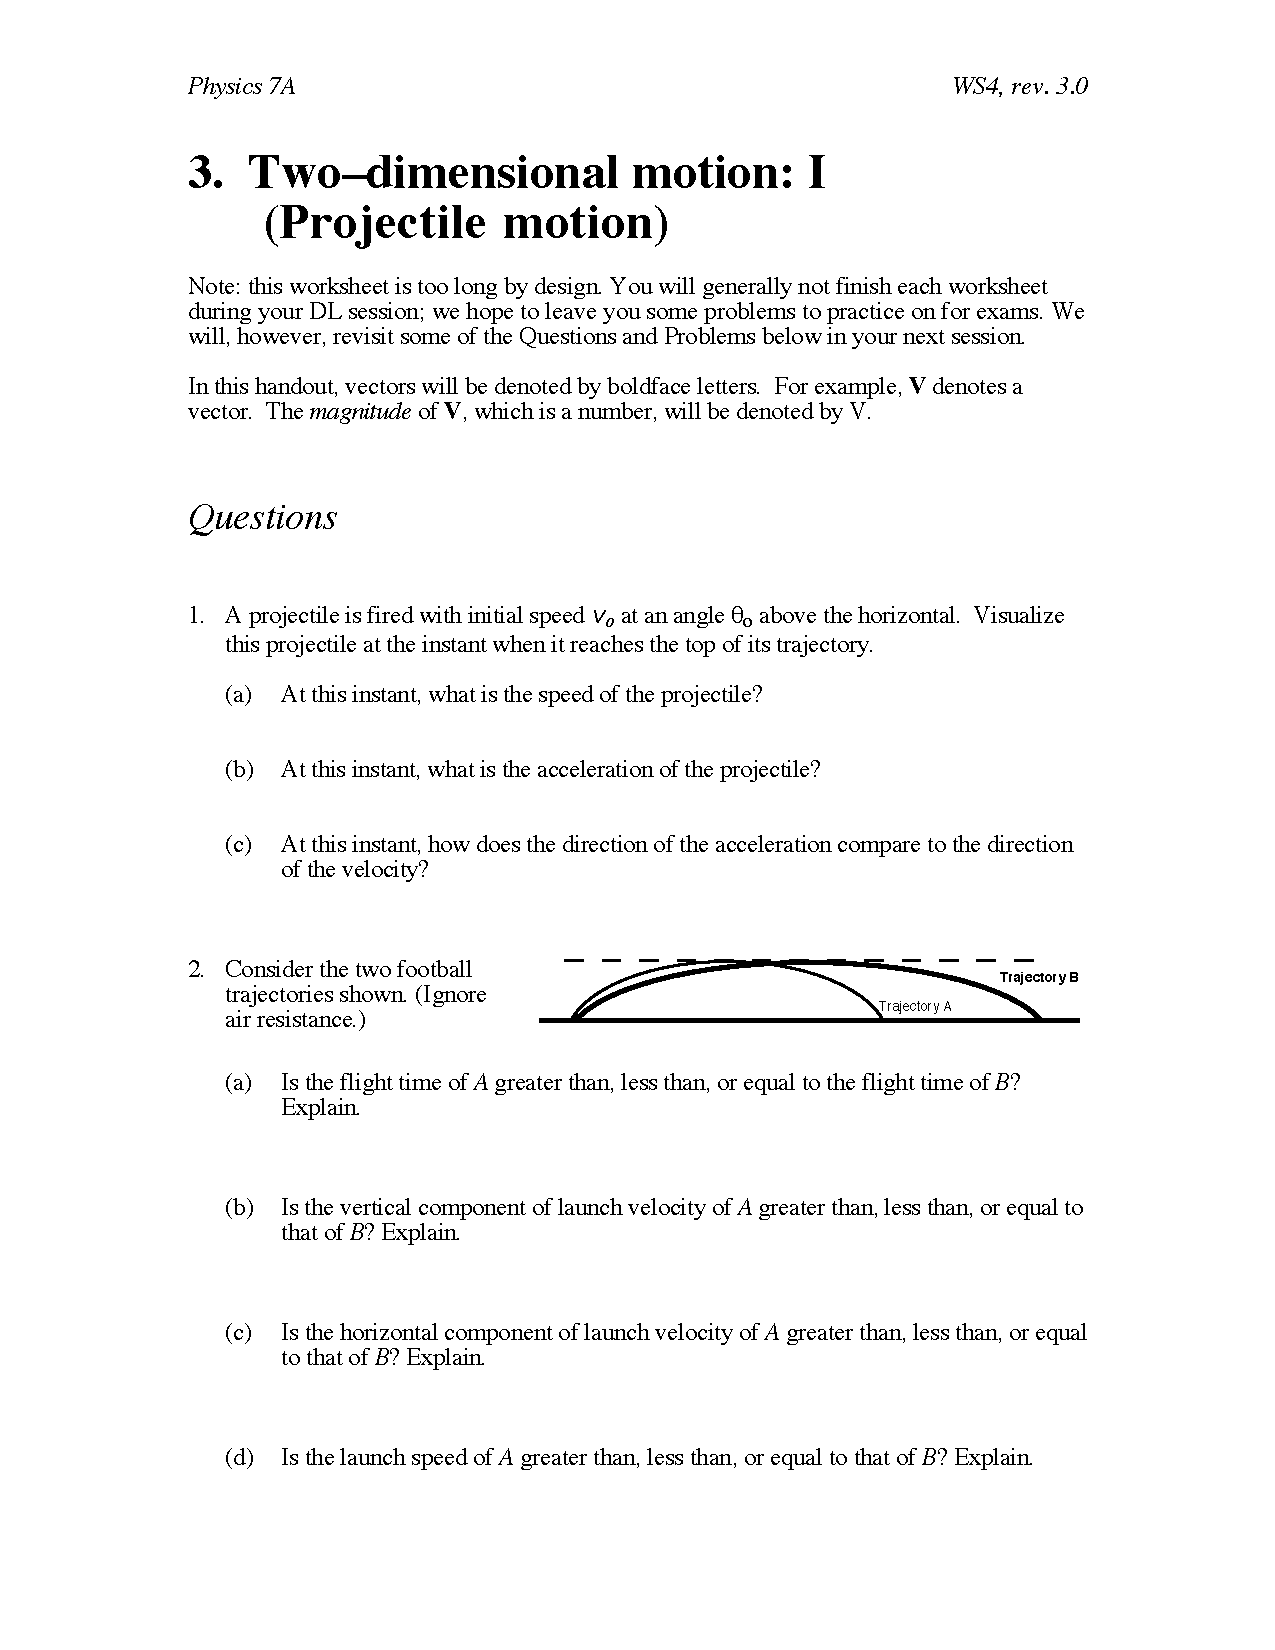
\includepdf[pages=-]{figs/0620/wb1718.pdf}

\section{Projectile Motion}

\textbf{1.} \textit{Giancoli, Physics for Scientists and Engineers, Problem 3.51} \\
A ball is thrown horizontally from the top of a cliff with initial speed $v_0$ (at $t = 0$). At any moment, its direction of motion makes an angle $\theta$ to the horizontal. Derive a formula for $\theta$ as a function of time as the ball follows a projectile’s path. 
\fig{figs/0620/proj.png}{Giancoli, Problem 3.51}{0.75}{0}
\vspace{1 in}

\textbf{2.} \textit{Physics 7A Workbook, Problem 3.4 (Next Page)} 
\vspace{1 in}

\textbf{3-4.} \textit{Physics 7A Past Exam Problems (Next Two Pages)} 
\vspace{1 in}

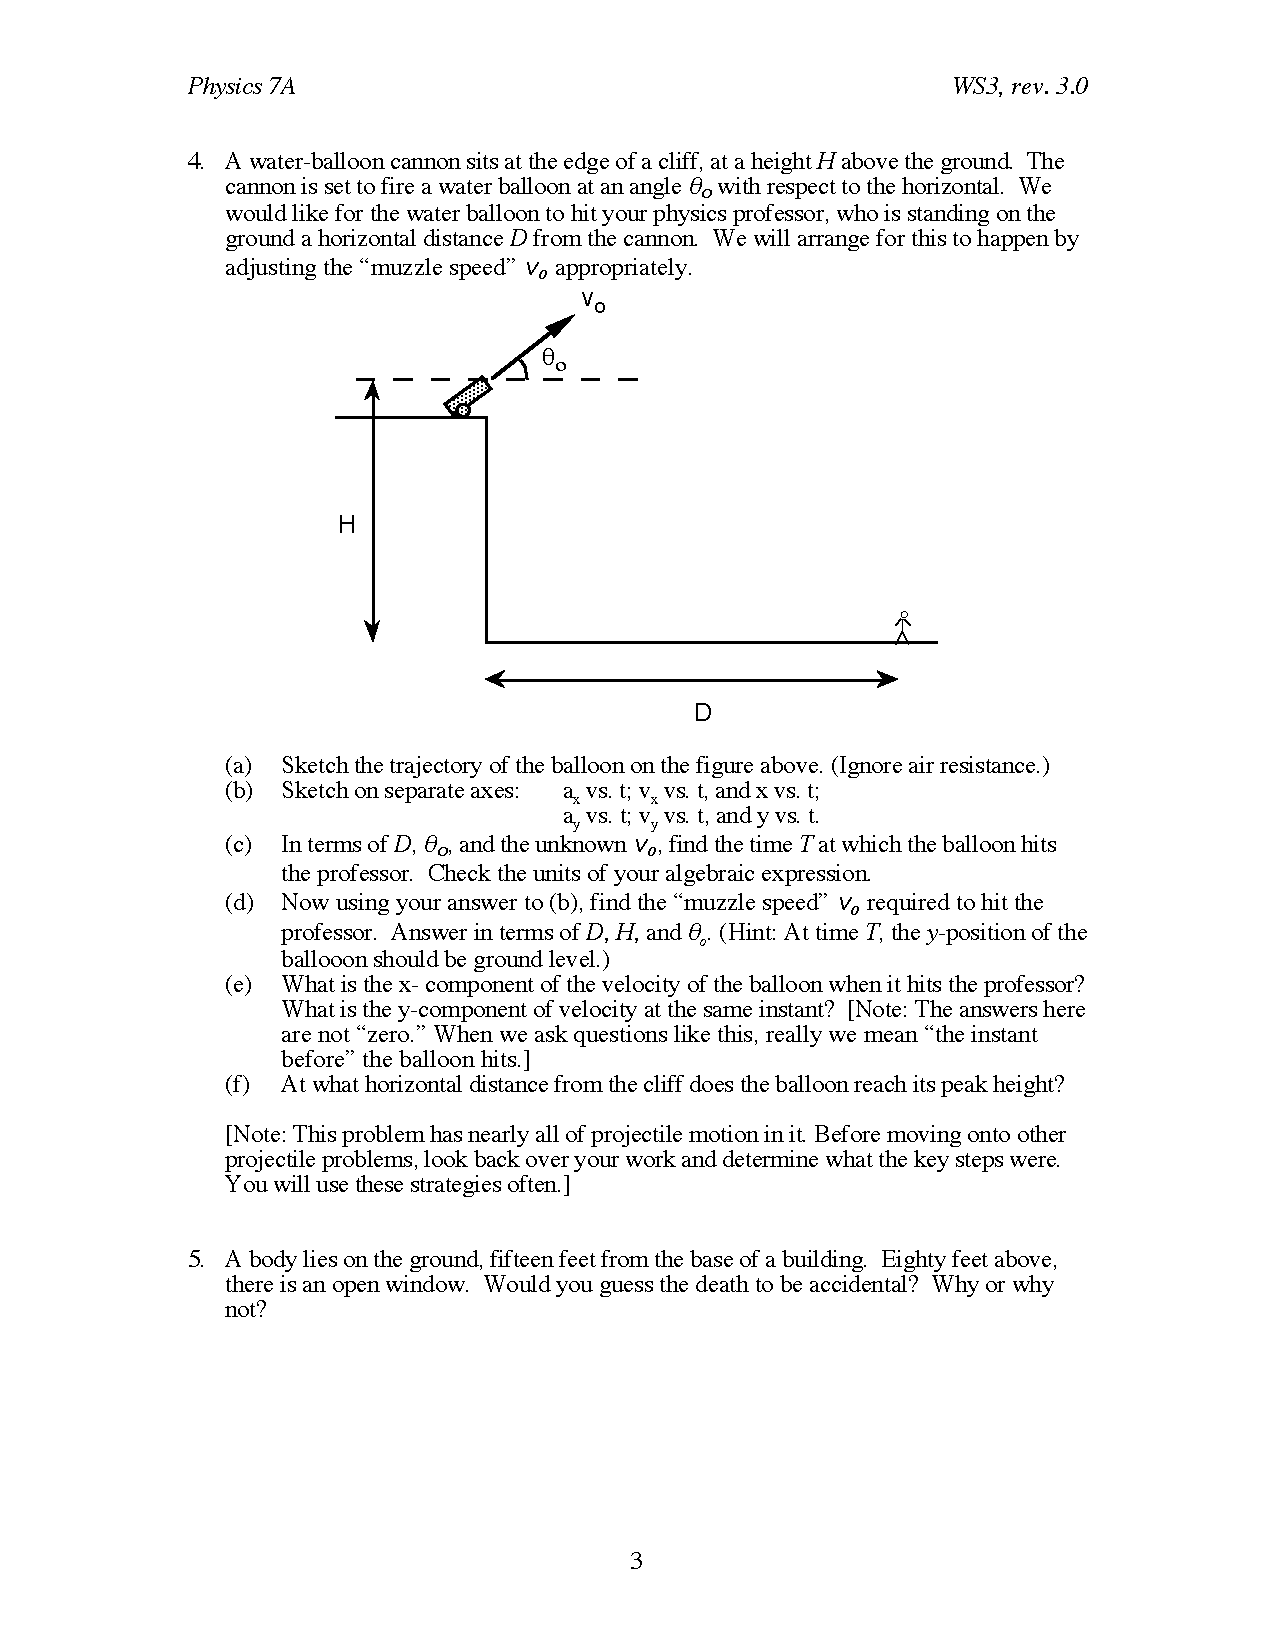
\includepdf[pages=-]{figs/0620/wb19.pdf}

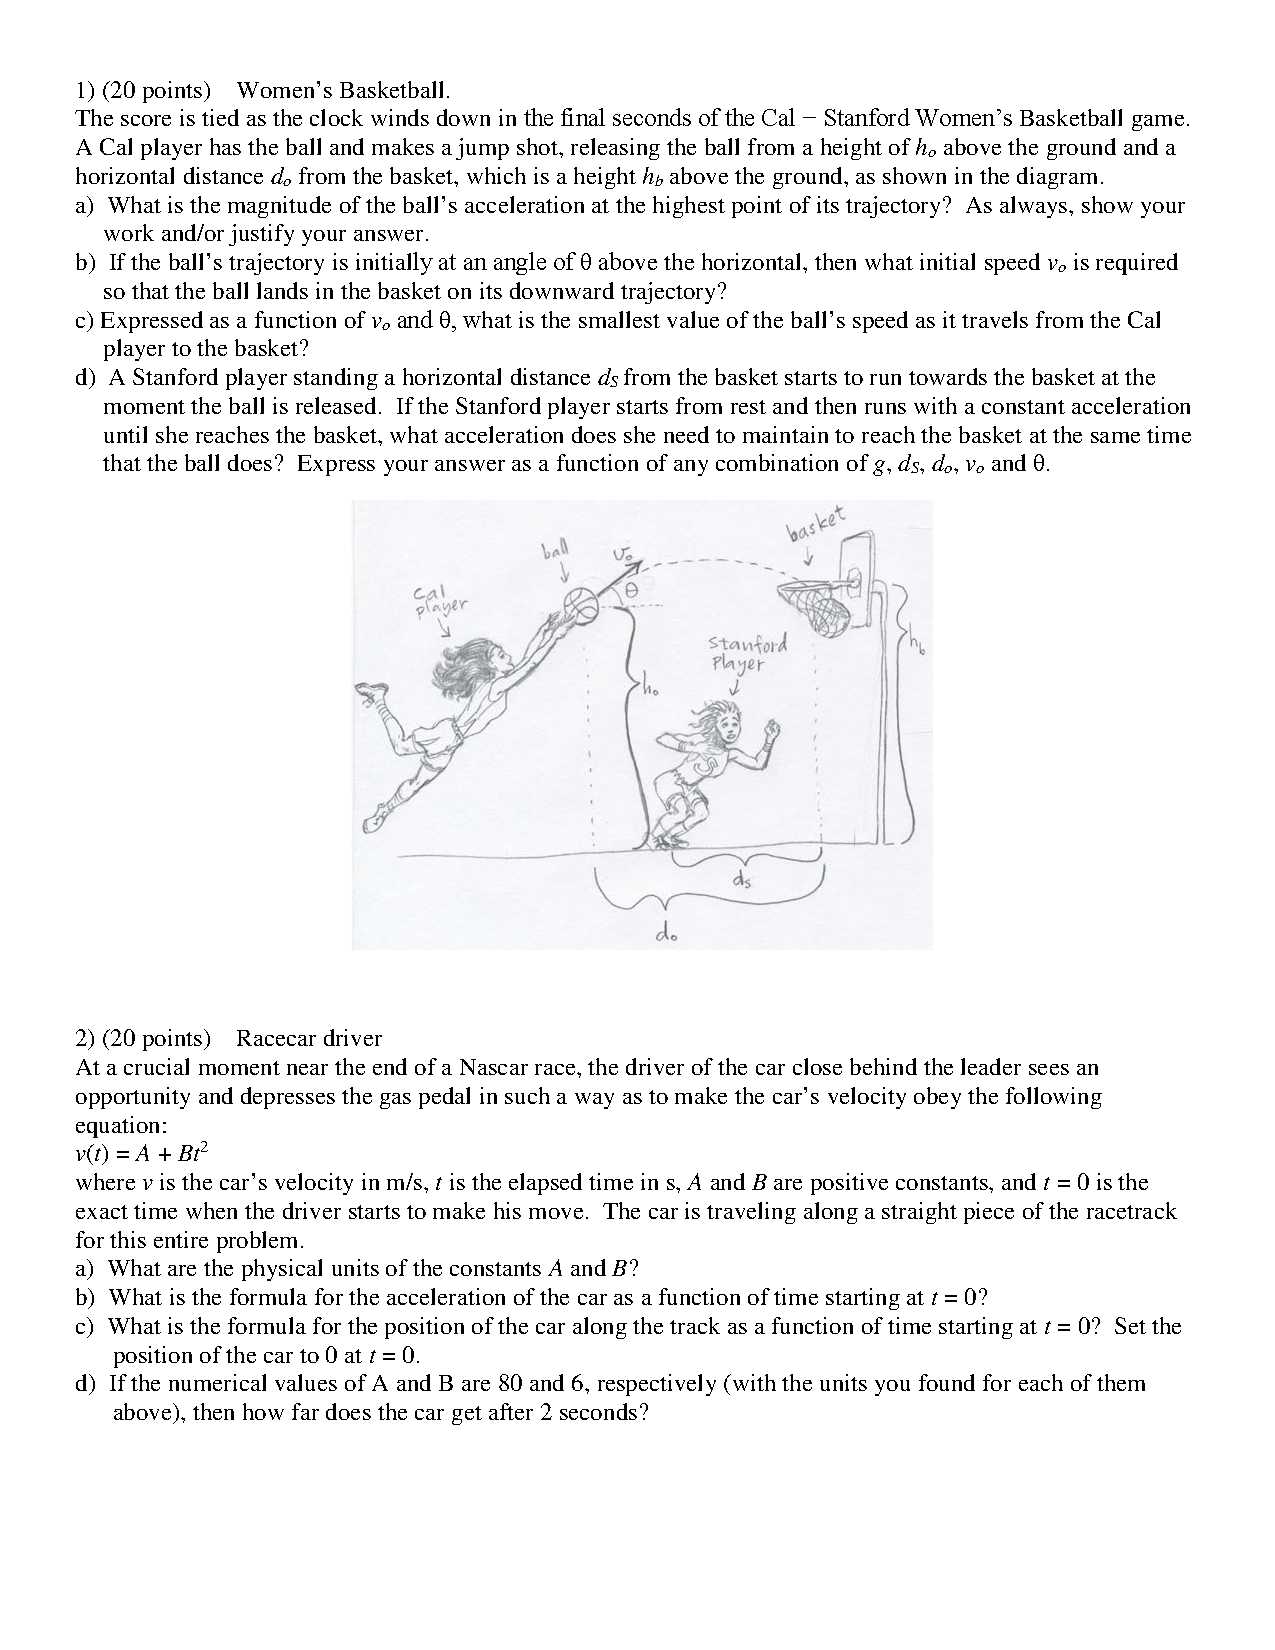
\includepdf[pages=-]{figs/0620/mt14.pdf}

\end{document}
